
\section{Specmine, an R package for metabolomics data analysis} \label{specmine_chapter}

As discussed in \autoref{met_tools}, most freely available tools are limited to specific types of metabolomics or spectral data and some offer a limited portfolio of data analysis tools for the construction of analysis pipelines. 

To address this problem, the R package \textit{specmine} was made available \citep{costa2016r}. It was developed under the R environment which is a free development environment for data manipulation, scientific and statistical computing and graphical visualization. \textit{Specmine} provides a set of methods for metabolomics and spectral data analysis, including data loading in various formats, data pre-processing, metabolite identification, univariate and multivariate data analysis, machine learning and also feature selection. 

The implemented methods allow for the analysis of metabolomics and spectral data, including \gls{gcms}, \gls{lcms}, \gls{nmr}, \gls{ir} and \gls{uv} data, integrating many available functions provided by other metabolomics oriented R packages and also more general-purpose data analysis R functions. Some of \textit{specmine} package dependencies include:

\begin{itemize}
	\item \textit{\textbf{hyperSpec}}: facilitates hyperspectral data sets handling (i.e. spatially or time-resolved spectra, which may consist of any data that is recorded over a discretized variable);
	\item \textit{\textbf{ChemoSpec}}: a collection of functions for top-down exploratory data analysis of spectral data obtained via \gls{nmr}, \gls{ir} or Raman spectroscopy;
	\item \textit{\textbf{rgl}}: provides medium to high level functions for 3D interactive graphics;
	\item \textit{\textbf{ggplot2}}: a system for 'declaratively' creating graphics, based on "The Grammar of Graphics";
	\item \textit{\textbf{caret}}: miscellaneous functions for training and plotting classification and regression models.
\end{itemize}

Besides providing a tool that covers the main metabolomics and spectral data types, \textit{specmine} also addresses a full range of tasks in data analysis, allowing for the creation of flexible and powerful analysis pipelines for specific case studies, providing abundant graphical visualization of the results. \autoref{specmine} shows the modules present in this package. Since metabolite identification is not usually the goal in a metabolic fingerprinting approach, which is emphasized throughout this dissertation, the metabolite identification module won't be discussed here.

\begin{figure}[!htb]
	\centering
	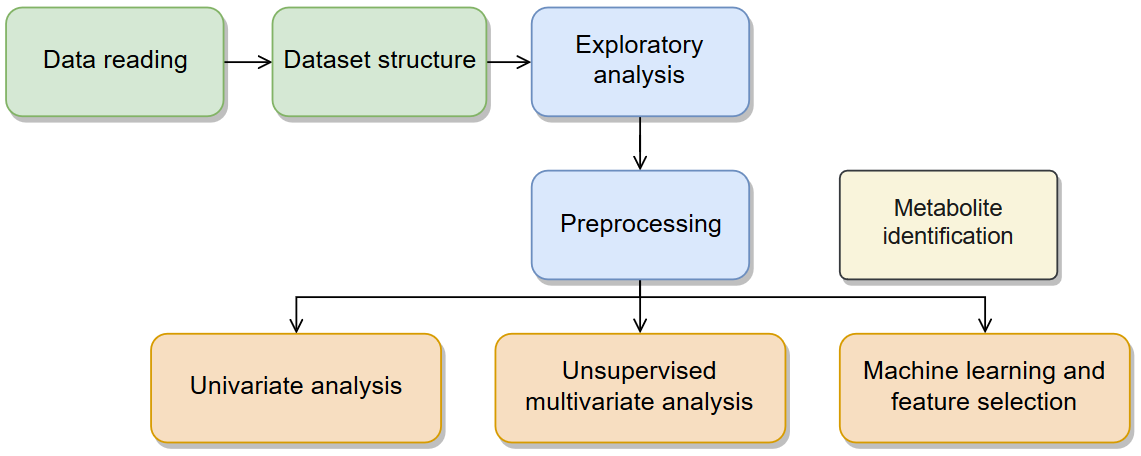
\includegraphics[width=0.85\linewidth]{Imagens/specmine}
	\caption{Modules in the \textit{specmine} package. Adapted from \cite{costa2016r}.}
	\label{specmine}
\end{figure}

\subsection{Data reading and dataset structure}

\textit{Specmine} supports a number of different file formats, including comma (or tab) separated values (CSV or TSV) files, (J)DX spectra files, NetCDF, mzDATA and mzXMLMS data. The metadata file can be given in the CSV/TSV format. Data can also be loaded as a peaks list, which are converted into a dataset using peak alignment functions. 

The structure of the dataset used in this package is independent of the data type and source and consists in an R list with the following fields: description of the dataset, the type of data, the data matrix, the metadata data frame and the labels for the x and y-axis. A graphical representation of the dataset structure is represented in \autoref{datas_tructure}.


\begin{figure}[!htb]
	\centering
	\includegraphics[width=0.9\linewidth]{Imagens/data_structure}
	\caption{Representation of the dataset structure in \textit{specmine}. Adapted from \cite{costa2016r}.}
	\label{datas_tructure}
\end{figure}

A list of all \textit{specmine} functions regarding data reading and dataset structure is shown in \autoref{specmine_functions_data_reading}.

\begin{scriptsize}
	\begin{longtable}{|m{4.3cm}|m{10cm}|}
		%FIRST HEADER------
		\caption{\textit{Specmine} package functions regarding data reading and dataset structure} 
		\label{specmine_functions_data_reading} \\
		\rowcolor{airforceblue}
		\htab{Function name} & \htab{Description} \\
		\hline
		\endfirsthead
		
		%SECOND HEADER------
		\caption[]{\textit{Specmine} package functions regarding data reading and dataset structure. (Continued)} \\
		\rowcolor{airforceblue}
		\htab{Function name} & \htab{Description} \\
		\hline
		\endhead
		
		%TABLE--------------
		
		\hline
		check\_dataset & Check if the dataset is valid and if not give the proper error message. \\
		
		\hline
		convert\_from\_chemospec & Convert the dataset in the ChemoSpec format to a dataset of this package. \\
		
		\hline
		convert\_from\_hyperspec & Convert the dataset in the hyperspec format to a dataset of this package. \\
		
		\hline
		convert\_to\_hyperspec & Convert a dataset to an hyperspec object. \\
		
		\hline
		create\_dataset & Create a dataset from existing objects \\
		
		\hline
		dataset\_from\_peaks & Converts a peak list to a dataset. \\
		
		\hline
		is\_spectra & Check if the dataset is from spectral data where x.values are numeric. \\
		
		\hline
		read\_csvs\_folder & Reads multiple CSV files in a given folder. \\
		
		\hline
		read\_dataset\_csv & Reads the data from a CSV file and creates the dataset. \\
		
		\hline
		read\_dataset\_dx & Reads the data from the (J)DX files and creates the dataset. \\
		
		\hline
		read\_dataset\_spc & Reads the data from the SPC files and creates the dataset. \\
		
		\hline
		read\_data\_csv & Reads the data from the CSV file. \\
		
		\hline
		read\_data\_dx & Reads the data from the (J)DX files. \\
		
		\hline
		read\_data\_spc & Reads the data from the SPC files. \\
		
		\hline
		read\_metadata & Read the metadata from a file. \\
		
		\hline
		read\_ms\_spectra & Read the data from the MS files and creates the dataset. \\
		
		\hline
		read\_multiple\_csvs & Reads multiple CSVs, each one with a sample. \\
		
		\hline
		
	\end{longtable}
\end{scriptsize}

\subsection{Exploratory analysis and data pre-processing}

\textit{Specmine} includes functions that allow to calculate global statistics and visualize the data in a graphical way. The package can calculate the main descriptive statistics over the data matrix of a dataset for both variables and samples, having functions that can be applied over the entire dataset or to a subset of samples or variables. Graphical visualization of the data is done for instance in the form of boxplots, which allows to see the distribution of values for a set of variables. The package also provides functions for spectra plotting, where the variables are represented by numerical values. Visualization functions rely on both ggplot2 and the base graphics system of R.

Preprocessing methods are also provided for the different types of data. They include methods for extracting relevant parts of a dataset, namely subsets of samples, data and metadata variables. Spectral pre-processing methods include functions for shifting correction, multiplicative scatter correction, first derivative, baseline, offset and background corrections. Some methods for smoothing interpolation are also available, including bin or loess smoothing, as well as Savitzky-Golay filters. Missing values can be treated by either removing samples and/or variables that have a number of missing values above a given threshold or replaced using a variety of different methods. 

Specmine also includes functions for data normalization, which can be done by sum, median, a reference sample or feature, for data transformation using cubic root and logarithmic methods, and scaling using auto, range and pareto methods. The package also provides flat pattern filters with distinct metrics and parameters that allow to remove variables with low variance. The various \textit{specmine} functions for data exploratory analysis and pre-processing are listed in \autoref{specmine_functions_prepocessing}.

\begin{scriptsize}
	\begin{longtable}{|m{4.3cm}|m{11cm}|}
		%FIRST HEADER------
		\caption{\textit{Specmine} package functions for data exploratory analysis and pre-processing.} 
		\label{specmine_functions_prepocessing} \\
		\rowcolor{airforceblue}
		\htab{Function name} & \htab{Description} \\
		\hline
		\endfirsthead
		
		%SECOND HEADER------
		\caption[]{\textit{Specmine} package functions for data exploratory analysis and pre-processing. (Continued)} \\
		\rowcolor{airforceblue}
		\htab{Function name} & \htab{Description} \\
		\hline
		\endhead
		
		%TABLE--------------
		
		\hline
		absorbance\_to\_transmittance & Converts absorbance values to transmittance values. \\
		
		\hline
		aggregate\_samples & Aggregate samples according to an aggregate function like mean, median, etc. \\
		
		\hline
		apply\_by\_group & Apply a function to samples from a given metadata's group. \\
		
		\hline
		apply\_by\_groups & Apply a function to samples from a metadata's variable. \\
		
		\hline
		apply\_by\_sample & Applies a function to the values of each sample \\
		
		\hline
		apply\_by\_variable & Applies a function to the values of each variable \\
		
		\hline
		background\_correction & Perform background correction on the spectra. \\
		
		\hline
		baseline\_correction & Performs baseline correction on the dataset. \\
		
		\hline
		boxplot\_variables & Boxplot of each variable of the dataset. \\
		
		\hline
		boxplot\_vars\_factor & Boxplot of variables with metadata's variable factors from the dataset. \\
		
		\hline
		compare\_regions\_by\_sample & Compare two regions of a dataset by samples. \\
		
		\hline
		convert\_to\_factor & Convert a metadata's variable to factor. \\
		
		\hline
		count\_missing\_values & Counts the missing values on the dataset. \\
		
		\hline
		count\_missing\_values\_per\_sample & Counts the missing values on each sample of the dataset. \\
		
		\hline
		count\_missing\_values\_per\_variable & Counts the missing values on each variable of the dataset. \\
		
		\hline
		cubic\_root\_transform & Performs cubic root transformation on the data matrix. \\
		
		\hline
		data\_correction & Perform spectra corrections with 3 different methods. \\
		
		\hline
		find\_equal\_samples & Finds samples that have the same peak values - $ x $ and $ y $ (equal data frames) \\
		
		\hline
		first\_derivative & Calculates the first derivative of the data. \\
		
		\hline
		get\_data & Get the data matrix from dataset \\
		
		\hline
		get\_data\_as\_df & Get the data matrix from the dataset as a data frame. \\
		
		\hline
		get\_data\_value & Get a data value given the x-axis labels and the sample \\
		
		\hline
		get\_data\_values & Gets the values of all samples in the dataset given a set of x axis names or indexes. \\
		
		\hline
		get\_metadata & Get the metadata from the dataset \\
		
		\hline
		get\_metadata\_value & Get the metadata value \\
		
		\hline
		get\_metadata\_var & Get the values of a metadata variable from the dataset. \\
		
		\hline
		get\_peak\_values & Gets the peak values from a data frame of samples’ peaks. \\
		
		\hline
		get\_samples\_names\_dx & Function to get the names of the DX files from a folder. \\
		
		\hline
		get\_samples\_names\_spc & Function to get the names of the SPC files from a folder. \\
		
		\hline
		get\_sample\_names & Get the sample names from the dataset. \\
		
		\hline
		get\_type & Get the type of the data from the dataset \\
		
		\hline
		get\_value\_label & Get the value label from the dataset \\
		
		\hline
		get\_x\_label & Get the x-axis label from the dataset. \\
		
		\hline
		get\_x\_values\_as\_num & Get the x-axis values from the dataset as numbers. \\
		
		\hline
		get\_x\_values\_as\_text & Get the x-axis values from the dataset as text. \\
		
		\hline
		group\_peaks & Group peaks with peak alignment. \\
		
		\hline
		impute\_nas\_knn & Impute missing values with KNN \\
		
		\hline
		impute\_nas\_linapprox & Impute missing values with linear approximation. \\
		
		\hline
		impute\_nas\_mean & Impute missing values with mean \\
		
		\hline
		impute\_nas\_median & Impute missing values with median \\
		
		\hline
		impute\_nas\_value & Impute missing values with value replacement. \\
		
		\hline
		indexes\_to\_xvalue\_interval & Returns x-values corresponding to a vector of indexes (only to numerical values - spectra) \\
		
		\hline
		log\_transform & Performs logarithmic transformation on the data matrix. \\
		
		\hline
		low\_level\_fusion & Low level fusion method for integrate different datasets (only samples with the same name on all
		datasets will be merged) \\
		
		\hline
		mean\_centering & Performs mean centering on the dataset. \\
		
		\hline
		merge\_datasets & Merges two datasets with the same variables and metadata’s variables. \\
		
		\hline
		merge\_data\_metadata & Merges the data and metadata from the dataset into a single data.frame. \\
		
		\hline
		metadata\_as\_variables & Use one or more metadata variables as variables. \\
		
		\hline
		missingvalues\_imputation & Treats the missing values of a dataset according to a specific method. \\
		
		\hline
		msc\_correction & Perform multiplicative scatter correction on the spectra. \\
		
		\hline
		multiplot & Multiplot from \textit{ggplot2} package \\
		
		\hline
		normalize & Normalize the data from the dataset with a specific method. \\
		
		\hline
		normalize\_samples & Normalize the data from a datamatrix with a specific method. \\
		
		\hline
		num\_samples & Get the number of samples from a dataset. \\
		
		\hline
		num\_x\_values & Get the number of x-axis values. \\
		
		\hline
		offset\_correction & Perform offset correction on the data. \\
		
		\hline
		peaks\_per\_sample & Counts number of peaks in a sample (given its index). \\
		
		\hline
		peaks\_per\_samples & Calculates the number of peaks on each sample. \\
		
		\hline
		plotvar\_twofactor & Plot variable distribution on two factors from the dataset. \\
		
		\hline
		plot\_spectra & Plot spectra from dataset. \\
		
		\hline
		plot\_spectra\_simple & Plot spectra from dataset (simple version). \\
		
		\hline
		remove\_data & Remove data from the dataset. \\
		
		\hline
		remove\_data\_variables & Remove data variables from the dataset. \\
		
		\hline
		remove\_metadata\_variables & Remove metadata's variables from the dataset \\
		
		\hline
		remove\_peaks\_interval & Removes peaks from a given interval. \\
		
		\hline
		remove\_peaks\_interval\_sample\_list & Removes peaks on a sample list given a peak interval. \\
		
		\hline
		remove\_samples & Remove samples from the dataset. \\
		
		\hline
		remove\_samples\_by\_nas & Remove samples from the dataset by the number of NAs \\
		
		\hline
		remove\_samples\_by\_na\_metadata & Remove samples from the dataset with the metadata's variable value with NAs. \\
		
		\hline
		remove\_variables\_by\_nas & Remove variables from the dataset by the number of NAs \\
		
		\hline
		remove\_x\_values\_by\_interval & Remove an interval of x-values from the dataset. \\
		
		\hline
		replace\_data\_value & Replace a data value for a new value on the dataset. \\
		
		\hline
		replace\_metadata\_value & Replace a metadata’s variable value of a sample. \\
		
		\hline
		savitzky\_golay & Smoothing and derivative of the data using Savitzky-Golay. \\
		
		\hline
		scaling & Performs scaling according to a method. \\
		
		\hline
		scaling\_samples & Performs scaling according to a method. \\
		
		\hline
		set\_metadata & Updates the dataset’s metadata with a new one. \\
		
		\hline
		set\_sample\_names & Set new samples names to the dataset. \\
		
		\hline
		set\_value\_label & Set a new value label for the dataset. \\
		
		\hline
		set\_x\_label & Set a new x-label to the dataset. \\
		
		\hline
		set\_x\_values & Set new x-values to the dataset \\
		
		\hline
		shift\_correction & Shifts the spectra according to a specific method. \\
		
		\hline
		smoothing\_interpolation & Performs smoothing interpolation according to a specific method. \\
		
		\hline
		snv\_dataset & Performs Standard Normal Variate on the dataset. \\
		
		\hline
		stats\_by\_sample & Get a summary of statistics of the samples. \\
		
		\hline
		stats\_by\_variable & Get a summary of statistics of the variables. \\
		
		\hline
		subset\_by\_samples\_and\_xvalues & Gets a subset of specific samples and x-values. \\
		
		\hline
		subset\_metadata & Subsets the metadata according to the specified metadata's variables. \\
		
		\hline
		subset\_random\_samples & Gets a subset of random samples from the dataset. \\
		
		\hline
		subset\_samples & Gets a subset of specific samples from the dataset. \\
		
		\hline
		subset\_samples\_by\_metadata\_values & Gets a subset of specific samples according to metadata’s values from the dataset. \\
		
		\hline
		subset\_x\_values & Gets a subset of specific x-values from the dataset. \\
		
		\hline
		subset\_x\_values\_by\_interval & Gets a subset of a specific interval of x-values. \\
		
		\hline
		sum\_dataset & Returns a summary with its main features. \\
		
		\hline
		transform\_data & Performs data transformation according to a method. \\
		
		\hline
		transmittance\_to\_absorbance & Converts transmittance values to absorbance values. \\
		
		\hline
		values\_per\_peak & Gets the number of values on each peak. \\
		
		\hline
		values\_per\_sample & Gets the number of values on each sample. \\
		
		\hline
		variables\_as\_metadata & Use one or more data variables as metadata variables. \\
		
		\hline
		xvalue\_interval\_to\_indexes & Returns indexes corresponding to an interval of x-values (only to numerical values - spectra) \\
		
		\hline
		x\_values\_to\_indexes & Returns the indexes corresponding to a vector of x-values (only to numerical values - spectra) \\
		
		\hline
		
	\end{longtable}
\end{scriptsize}


\subsection{Univariate and unsupervised multivariate analysis}

For univariate analysis, \textit{specmine} offers a set of functions that cover various analysis types such as t-tests, \gls{anova}, regression analysis, correlations and \gls{fc} calculation. The package offers one-way \gls{anova}, with the TukeyHSD post hoc test, and also multifactorial \gls{anova}, with functions to summarize the main results, including p-values and the percentage of variation explained by the different factors. These p-values are already adjusted using the \gls{fdr} method. Non-parametric tests include the Kruskal-Wallis and Kolmogorov-Smirnov tests. 

For the linear regression analysis \textit{specmine} offers functions that summarize the coefficients for the different factors and interactions and respective p-values. The correlations between variables or samples can be computed and the resulting matrix visualized as a heatmap. For \gls{fc} analysis the package offers functions to calculate the fold changes of values considering two groups of samples, and the results can be visualized in both tabular and graphical forms, similarly to the t-tests results.
 
As for the unsupervised multivariate analysis \textit{specmine} provides functions to perform \gls{pca} using two methods: classical and robust, where the latter makes use of the grid search algorithm to compute the desired number of principal components. The results of \gls{pca} can be visualized through a variety of graphs, including scree plots, scores plots, biplots and pairs plots. 

The package also offers functions to perform k-means and hierarchical clustering methods. The distance method to use can be chosen as well as the method to use in the case of hierarchical clustering. K-means clustering results can be plotted in the form of a graph with the k clusters in different colors and hierarchical clustering results plotted as a dendogram. The various \textit{specmine} functions for univariate and unsupervised multivariate analysis are listed in \autoref{specmine_functions_analysis}.



\begin{scriptsize}
	\begin{longtable}{|m{4.3cm}|m{11cm}|}
		%FIRST HEADER------
		\caption{\textit{Specmine} package functions for univariate and unsupervised multivariate analysis.} 
		\label{specmine_functions_analysis} \\
		\rowcolor{airforceblue}
		\htab{Function name} & \htab{Description} \\
		\hline
		\endfirsthead
		
		%SECOND HEADER------
		\caption[]{\textit{Specmine} package functions for univariate and unsupervised multivariate analysis. (Continued)} \\
		\rowcolor{airforceblue}
		\htab{Function name} & \htab{Description} \\
		\hline
		\endhead
		
		%TABLE--------------
		
		\hline
		aov\_all\_vars & Perform analysis of variance of all variables in the dataset. \\
		
		\hline
		clustering & Perform cluster analysis on the dataset. \\
		
		\hline
		correlations\_dataset & Calculate the correlations of all variables or samples in the dataset. \\
		
		\hline
		correlations\_test & Performs correlations test to the whole dataset. \\
		
		\hline
		correlation\_test & Performs correlations test of two variables or samples from the dataset. \\
		
		\hline
		dendrogram\_plot & Plot dendrogram of hierarchical clustering results. \\
		
		\hline
		dendrogram\_plot\_col & Plot dendrogram of hierarchical clustering results with different colors \\
		
		\hline
		fold\_change & Perform fold change analysis on the dataset. \\
		
		\hline
		fold\_change\_var & Fold change applied on two variables. Instead of having the difference of the variables on two
		groups, we have the difference of the groups on two variables. \\
		
		\hline
		heatmap\_correlations & Plots a heatmap with the correlations. \\
		
		\hline
		hierarchical\_clustering & Perform hierarchical clustering analysis on the dataset. \\
		
		\hline
		kmeans\_clustering & Perform k-means clustering analysis on the dataset. \\
		
		\hline
		kmeans\_plot & Plot for each formed cluster, in grey the values of all samples of that cluster and in blue the median
		of that samples. \\
		
		\hline
		kmeans\_result\_df & Show for each cluster from kmeans analysis the sample names belonging to them. \\
		
		\hline
		kruskalTest\_dataset & Run Kruskal-Wallis Tests for each row of the data from the dataset. \\
		
		\hline
		ksTest\_dataset & Run Kolmogorov-Smirnov Tests for each row of the data from the dataset. \\
		
		\hline
		linregression\_onevar & Performs linear regression on one variable of the dataset. \\
		
		\hline
		linreg\_all\_vars & Performs linear regression analysis over the dataset with the selected metadata’s variables. \\
		
		\hline
		linreg\_coef\_table & Gets a data.frame with the coefficient values. \\
		
		\hline
		linreg\_pvalue\_table & Gets the p-values table from the linear regression analysis. \\
		
		\hline
		linreg\_rsquared & Gets the linear regression r-squared values. \\
		
		\hline
		multifactor\_aov\_all\_vars & Perform multi-factor ANOVA on all variables with the selected metadata variables. \\
		
		\hline
		multifactor\_aov\_pvalues\_table & Gets the p-values table from the multifactor ANOVA results. \\
		
		\hline
		multifactor\_aov\_varexp\_table & Gets the variability explained table from the multifactor ANOVA results. \\
		
		\hline
		pca\_analysis\_dataset & Performs a classical PCA analysis over the dataset. \\
		
		\hline
		pca\_biplot & Shows a PCA biplot. \\
		
		\hline
		pca\_biplot3D & Shows a interactive 3D PCA biplot. \\
		
		\hline 
		pca\_importance & Gets the importance from the PCs. \\
		
		\hline
		pca\_kmeans\_plot2D & Groups the points with the clusters given by k-means in a 2D PCA scores plot. \\
		
		\hline
		pca\_kmeans\_plot3D & Groups the points with the clusters given by k-means in a interactive 3D PCA scores plot. \\
		
		\hline
		pca\_pairs\_kmeans\_plot & Groups the points with the clusters from k-means in a PCA pairs plot. \\
		
		\hline
		pca\_pairs\_plot & Shows a PCA pairs plot. \\
		
		\hline
		pca\_plot\_3d & 3D plot from 3 components \\
		
		\hline
		pca\_robust & Performs a robust PCA analysis. \\
		
		\hline
		pca\_scoresplot2D & Shows a 2D PCA scores plot of two principal componets. \\
		
		\hline
		pca\_scoresplot3D & Shows a 3D PCA scores plot of three principal componets. \\
		
		\hline
		pca\_scoresplot3D\_rgl & Shows a interactive 3D PCA scores plot of three principal components. \\
		
		\hline
		pca\_screeplot & PCA scree plot with the proportion and cumulative variance of the PCs. \\
		
		\hline
		plot\_anova & Function for plotting the results from ANOVA.
		Usage \\
		
		\hline
		plot\_fold\_change & Function for plotting the results from fold change. \\
		
		\hline
		plot\_kruskaltest & Function for plotting the results from Kruskal-Wallis tests. \\
		
		\hline
		plot\_kstest & Function for plotting the results from Kolmogorov-Smirnov tests. \\
		
		\hline
		plot\_regression\_coefs\_pvalues & Plots the linear regression coefficient and the p-values. \\
		
		\hline
		plot\_ttests & Function for plotting the results from t-tests. \\
		
		\hline
		tTests\_dataset & Run t-Tests for each row of the data from the dataset. \\
		
		\hline
		volcano\_plot\_fc\_tt & Volcano plot to intersect the results from t-tests and fold change. \\
		
		\hline
		
	\end{longtable}
\end{scriptsize}


\subsection{Machine learning and feature selection}

For machine learning, the package offers a number of functions to train, use and evaluate the different methods, covering both classification and regression approaches. It also includes validation methods to estimate the error metrics, including k-fold cross-validation, leave-one-out cross-validation and resampling methods, among others. The error metrics available include accuracy, \gls{auc} and kappa statistic for classification, and \gls{rmse} and the coefficient of determination ($ R^{2} $) for regression. Functions to optimize model parameters (e.g. hidden nodes in a neural network) by testing and evaluating different values, according to the selected validation method and error metrics, are also available. This model optimization process gives the best model obtained and its performance, the variables’ importance, the results of all tested combinations of parameters, the confusion matrices (in the case of classification), among other statistics. The resulting trained models can then be used for new data prediction.

Feature selection methods provided by \textit{specmine} include both filter and wrapper methods, which can be combined with the machine learning methods. The package includes the most commonly used wrapper method \gls{rfe}, which tests different subsets of features, iteratively reducing the number of features and verifying which configuration provides the best performance. The various \textit{specmine} functions for machine learning and feature selection are listed in \autoref{specmine_functions_machine_learning}.


\begin{scriptsize}
	\begin{longtable}{|m{4.3cm}|m{11cm}|}
		%FIRST HEADER------
		\caption{\textit{Specmine} package functions for machine learning and feature selection.} 
		\label{specmine_functions_machine_learning} \\
		\rowcolor{airforceblue}
		\htab{Function name} & \htab{Description} \\
		\hline
		\endfirsthead
		
		%SECOND HEADER------
		\caption[]{\textit{Specmine} package functions for machine learning and feature selection. (Continued)} \\
		\rowcolor{airforceblue}
		\htab{Function name} & \htab{Description} \\
		\hline
		\endhead
		
		%TABLE--------------
		
		\hline
		feature\_selection & Perform feature selection on the dataset. \\
		
		\hline
		filter\_feature\_selection & Perform selection by filter using univariate filters, from \textit{caret}'s package. \\
		
		\hline
		flat\_pattern\_filter & Performs a flat pattern filter over the dataset. \\
		
		\hline
		multiClassSummary & Summary function for caret to compute AUC. \\
		
		\hline
		predict\_samples & Predict new samples. \\
		
		\hline
		recursive\_feature\_elimination & Perform recursive feature elimination on the dataset using \textit{caret}'s package. \\
		
		\hline
		summary\_var\_importance & Summary of variables importance of the models \\
		
		\hline
		train\_and\_predict & Train a model and predict new unlabeled samples with that model. \\
		
		\hline
		train\_classifier & Train a specific classifier. \\
		
		\hline
		train\_models\_performance & Train various models. \\
		
		\hline
		
	\end{longtable}
\end{scriptsize}




%\definecolor{moonstoneblue}{rgb}{0.64, 0.76, 0.68}
%
%\begin{scriptsize}
%	\begin{longtable}{|m{4.3cm}|m{11cm}|}
%		%FIRST HEADER------
%		\caption{\textit{Specmine} package functions.} 
%		\label{specmine_functions} \\
%		\rowcolor{airforceblue}
%		\htab{Function name} & \htab{Description} \\
%		\hline
%		\endfirsthead
%		
%		%SECOND HEADER------
%		\caption[]{\textit{Specmine} package functions. (Continued)} \\
%		\rowcolor{airforceblue}
%		\htab{Function name} & \htab{Description} \\
%		\hline
%		\endhead
%		
%		%TABLE--------------
%		
%		\hline
%		\rowcolor{moonstoneblue}
%		\multicolumn{2}{|l|}{\htab{Data reading and dataset structure}} \\ 
%		
%		 \hline
%		check\_dataset & Check if the dataset is valid and if not give the proper error message. \\
%								
%		\hline
%		convert\_from\_chemospec & Convert the dataset in the ChemoSpec format to a dataset of this package. \\
%		
%		\hline
%		convert\_from\_hyperspec & Convert the dataset in the hyperspec format to a dataset of this package. \\
%		
%		\hline
%		convert\_to\_hyperspec & Convert a dataset to an hyperspec object. \\
%						
%		\hline
%		create\_dataset & Create a dataset from existing objects \\
%		
%		\hline
%		dataset\_from\_peaks & Converts a peak list to a dataset. \\
%		
%		\hline
%		is\_spectra & Check if the dataset is from spectral data where x.values are numeric. \\
%		
%		\hline
%		read\_csvs\_folder & Reads multiple CSV files in a given folder. \\
%		
%		\hline
%		read\_dataset\_csv & Reads the data from a CSV file and creates the dataset. \\
%		
%		\hline
%		read\_dataset\_dx & Reads the data from the (J)DX files and creates the dataset. \\
%		
%		\hline
%		read\_dataset\_spc & Reads the data from the SPC files and creates the dataset. \\
%		
%		\hline
%		read\_data\_csv & Reads the data from the CSV file. \\
%		
%		\hline
%		read\_data\_dx & Reads the data from the (J)DX files. \\
%		
%		\hline
%		read\_data\_spc & Reads the data from the SPC files. \\
%		
%		\hline
%		read\_metadata & Read the metadata from a file. \\
%		
%		\hline
%		read\_ms\_spectra & Read the data from the MS files and creates the dataset. \\
%		
%		\hline
%		read\_multiple\_csvs & Reads multiple CSVs, each one with a sample. \\
%		
%		
%		% EXPLORATORY ANALYSIS AND PREPROCESSING
%		\hline
%		\rowcolor{moonstoneblue}
%		\multicolumn{2}{|l|}{\htab{Exploratory analysis and data pre-processing}} \\ 
%		
%		\hline
%		absorbance\_to\_transmittance & Converts absorbance values to transmittance values. \\
%		
%		\hline
%		aggregate\_samples & Aggregate samples according to an aggregate function like mean, median, etc. \\
%		
%		\hline
%		apply\_by\_group & Apply a function to samples from a given metadata's group. \\
%		
%		\hline
%		apply\_by\_groups & Apply a function to samples from a metadata's variable. \\
%		
%		\hline
%		apply\_by\_sample & Applies a function to the values of each sample \\
%								
%		\hline
%		apply\_by\_variable & Applies a function to the values of each variable \\
%		
%		\hline
%		background\_correction & Perform background correction on the spectra. \\
%		
%		\hline
%		baseline\_correction & Performs baseline correction on the dataset. \\
%		
%		\hline
%		boxplot\_variables & Boxplot of each variable of the dataset. \\
%		
%		\hline
%		boxplot\_vars\_factor & Boxplot of variables with metadata's variable factors from the dataset. \\
%		
%		\hline
%		compare\_regions\_by\_sample & Compare two regions of a dataset by samples. \\
%		
%		\hline
%		convert\_to\_factor & Convert a metadata's variable to factor. \\
%								
%		\hline
%		count\_missing\_values & Counts the missing values on the dataset. \\
%		
%		\hline
%		count\_missing\_values\_per\_sample & Counts the missing values on each sample of the dataset. \\
%		
%		\hline
%		count\_missing\_values\_per\_variable & Counts the missing values on each variable of the dataset. \\
%		
%		\hline
%		cubic\_root\_transform & Performs cubic root transformation on the data matrix. \\
%		
%		\hline
%		data\_correction & Perform spectra corrections with 3 different methods. \\
%		
%		\hline
%		\rowcolor{moonstoneblue}
%		\multicolumn{2}{|l|}{\htab{Exploratory analysis and data pre-processing}} \\ 
%		
%		\hline
%		find\_equal\_samples & Finds samples that have the same peak values - $ x $ and $ y $ (equal data frames) \\
%		
%		\hline
%		first\_derivative & Calculates the first derivative of the data. \\
%		
%		\hline
%		get\_data & Get the data matrix from dataset \\
%		
%		\hline
%		get\_data\_as\_df & Get the data matrix from the dataset as a data frame. \\
%		
%		\hline
%		get\_data\_value & Get a data value given the x-axis labels and the sample \\
%		
%		\hline
%		get\_data\_values & Gets the values of all samples in the dataset given a set of x axis names or indexes. \\
%		
%		\hline
%		get\_metadata & Get the metadata from the dataset \\
%		
%		\hline
%		get\_metadata\_value & Get the metadata value \\
%		
%		\hline
%		get\_metadata\_var & Get the values of a metadata variable from the dataset. \\
%		
%		\hline
%		get\_peak\_values & Gets the peak values from a data frame of samples’ peaks. \\
%								
%		\hline
%		get\_samples\_names\_dx & Function to get the names of the DX files from a folder. \\
%		
%		\hline
%		get\_samples\_names\_spc & Function to get the names of the SPC files from a folder. \\
%		
%		\hline
%		get\_sample\_names & Get the sample names from the dataset. \\
%								
%		\hline
%		get\_type & Get the type of the data from the dataset \\
%		
%		\hline
%		get\_value\_label & Get the value label from the dataset \\
%		
%		\hline
%		get\_x\_label & Get the x-axis label from the dataset. \\
%		
%		\hline
%		get\_x\_values\_as\_num & Get the x-axis values from the dataset as numbers. \\
%		
%		\hline
%		get\_x\_values\_as\_text & Get the x-axis values from the dataset as text. \\
%		
%		\hline
%		group\_peaks & Group peaks with peak alignment. \\
%		
%		\hline
%		impute\_nas\_knn & Impute missing values with KNN \\
%		
%		\hline
%		impute\_nas\_linapprox & Impute missing values with linear approximation. \\
%		
%		\hline
%		impute\_nas\_mean & Impute missing values with mean \\
%		
%		\hline
%		impute\_nas\_median & Impute missing values with median \\
%		
%		\hline
%		impute\_nas\_value & Impute missing values with value replacement. \\
%		
%		\hline
%		indexes\_to\_xvalue\_interval & Returns x-values corresponding to a vector of indexes (only to numerical values - spectra) \\
%		
%		\hline
%		log\_transform & Performs logarithmic transformation on the data matrix. \\
%								
%		\hline
%		low\_level\_fusion & Low level fusion method for integrate different datasets (only samples with the same name on all
%		datasets will be merged) \\
%		
%		\hline
%		mean\_centering & Performs mean centering on the dataset. \\
%		
%		\hline
%		merge\_datasets & Merges two datasets with the same variables and metadata’s variables. \\
%		
%		\hline
%		merge\_data\_metadata & Merges the data and metadata from the dataset into a single data.frame. \\
%		
%		\hline
%		metadata\_as\_variables & Use one or more metadata variables as variables. \\
%		
%		\hline
%		missingvalues\_imputation & Treats the missing values of a dataset according to a specific method. \\
%		
%		\hline
%		msc\_correction & Perform multiplicative scatter correction on the spectra. \\
%		
%		\hline
%		multiplot & Multiplot from \textit{ggplot2} package \\
%		
%		\hline
%		normalize & Normalize the data from the dataset with a specific method. \\
%		
%		\hline
%		normalize\_samples & Normalize the data from a datamatrix with a specific method. \\
%		
%		\hline
%		num\_samples & Get the number of samples from a dataset. \\
%		
%		\hline
%		num\_x\_values & Get the number of x-axis values. \\
%		
%		\hline
%		offset\_correction & Perform offset correction on the data. \\
%		
%		\hline
%		peaks\_per\_sample & Counts number of peaks in a sample (given its index). \\
%		
%		\hline
%	 	peaks\_per\_samples & Calculates the number of peaks on each sample. \\
%		
%		\hline
%		plotvar\_twofactor & Plot variable distribution on two factors from the dataset. \\
%		
%		\hline
%		plot\_spectra & Plot spectra from dataset. \\
%		
%		\hline
%		plot\_spectra\_simple & Plot spectra from dataset (simple version). \\
%		
%		\hline
%		remove\_data & Remove data from the dataset. \\
%		
%		\hline
%		remove\_data\_variables & Remove data variables from the dataset. \\
%		
%		\hline
%		\rowcolor{moonstoneblue}
%		\multicolumn{2}{|l|}{\htab{Exploratory analysis and data pre-processing}} \\ 
%		
%		\hline
%		remove\_metadata\_variables & Remove metadata's variables from the dataset \\
%		
%		\hline
%		remove\_peaks\_interval & Removes peaks from a given interval. \\
%		
%		\hline
%	 	remove\_peaks\_interval\_sample\_list & Removes peaks on a sample list given a peak interval. \\
%		
%		\hline
%		remove\_samples & Remove samples from the dataset. \\
%		
%		\hline
%		remove\_samples\_by\_nas & Remove samples from the dataset by the number of NAs \\
%		
%		\hline
%		remove\_samples\_by\_na\_metadata & Remove samples from the dataset with the metadata's variable value with NAs. \\
%		
%		\hline
%		remove\_variables\_by\_nas & Remove variables from the dataset by the number of NAs \\
%		
%		\hline
%		remove\_x\_values\_by\_interval & Remove an interval of x-values from the dataset. \\
%		
%		\hline
%		replace\_data\_value & Replace a data value for a new value on the dataset. \\
%		
%		\hline
%		replace\_metadata\_value & Replace a metadata’s variable value of a sample. \\
%		
%		\hline
%		savitzky\_golay & Smoothing and derivative of the data using Savitzky-Golay. \\
%		
%		\hline
%		scaling & Performs scaling according to a method. \\
%		
%		\hline
%		scaling\_samples & Performs scaling according to a method. \\
%		
%		\hline
%		set\_metadata & Updates the dataset’s metadata with a new one. \\
%		
%		\hline
%		set\_sample\_names & Set new samples names to the dataset. \\
%		
%		\hline
%	 	set\_value\_label & Set a new value label for the dataset. \\
%		
%		\hline
%		set\_x\_label & Set a new x-label to the dataset. \\
%		
%		\hline
%		set\_x\_values & Set new x-values to the dataset \\
%		
%		\hline
%		shift\_correction & Shifts the spectra according to a specific method. \\
%		
%		\hline
%		smoothing\_interpolation & Performs smoothing interpolation according to a specific method. \\
%		
%		\hline
%		snv\_dataset & Performs Standard Normal Variate on the dataset. \\
%		
%		\hline
%		stats\_by\_sample & Get a summary of statistics of the samples. \\
%		
%		\hline
%		stats\_by\_variable & Get a summary of statistics of the variables. \\
%		
%		\hline
%		subset\_by\_samples\_and\_xvalues & Gets a subset of specific samples and x-values. \\
%		
%		\hline
%		subset\_metadata & Subsets the metadata according to the specified metadata's variables. \\
%		
%		\hline
%		subset\_random\_samples & Gets a subset of random samples from the dataset. \\
%		
%		\hline
%		subset\_samples & Gets a subset of specific samples from the dataset. \\
%		
%		\hline
%		subset\_samples\_by\_metadata\_values & Gets a subset of specific samples according to metadata’s values from the dataset. \\
%		
%		\hline
%		subset\_x\_values & Gets a subset of specific x-values from the dataset. \\
%		
%		\hline
%		subset\_x\_values\_by\_interval & Gets a subset of a specific interval of x-values. \\
%		
%		\hline
%		sum\_dataset & Returns a summary with its main features. \\
%		
%		\hline
%		transform\_data & Performs data transformation according to a method. \\
%		
%		\hline
%		transmittance\_to\_absorbance & Converts transmittance values to absorbance values. \\
%		
%		\hline
%		values\_per\_peak & Gets the number of values on each peak. \\
%		
%		\hline
%		values\_per\_sample & Gets the number of values on each sample. \\
%		
%		\hline
%		variables\_as\_metadata & Use one or more data variables as metadata variables. \\
%		
%		\hline
%		xvalue\_interval\_to\_indexes & Returns indexes corresponding to an interval of x-values (only to numerical values - spectra) \\
%		
%		\hline
%		x\_values\_to\_indexes & Returns the indexes corresponding to a vector of x-values (only to numerical values - spectra) \\
%	
%		% UNIVARIATE ANALYSIS
%		\hline
%		\rowcolor{moonstoneblue}
%		\multicolumn{2}{|l|}{\htab{Univariate and unsupervised multivariate analysis}} \\ 
%				
%		\hline
%		aov\_all\_vars & Perform analysis of variance of all variables in the dataset. \\
%		
%		\hline
%		clustering & Perform cluster analysis on the dataset. \\
%		
%		\hline
%		correlations\_dataset & Calculate the correlations of all variables or samples in the dataset. \\
%		
%		\hline
%	 	correlations\_test & Performs correlations test to the whole dataset. \\
%						
%		\hline
%		correlation\_test & Performs correlations test of two variables or samples from the dataset. \\
%		
%		\hline
%		dendrogram\_plot & Plot dendrogram of hierarchical clustering results. \\
%		
%		\hline
%		dendrogram\_plot\_col & Plot dendrogram of hierarchical clustering results with different colors \\
%		
%		\hline
%		\rowcolor{moonstoneblue}
%		\multicolumn{2}{|l|}{\htab{Univariate and unsupervised multivariate analysis}} \\ 
%		
%		\hline
%		fold\_change & Perform fold change analysis on the dataset. \\
%		
%		\hline
%		fold\_change\_var & Fold change applied on two variables. Instead of having the difference of the variables on two
%		groups, we have the difference of the groups on two variables. \\
%		
%		\hline
%		heatmap\_correlations & Plots a heatmap with the correlations. \\
%		
%		\hline
%		hierarchical\_clustering & Perform hierarchical clustering analysis on the dataset. \\
%		
%		\hline
%		kmeans\_clustering & Perform k-means clustering analysis on the dataset. \\
%		
%		\hline
%		kmeans\_plot & Plot for each formed cluster, in grey the values of all samples of that cluster and in blue the median
%		of that samples. \\
%		
%		\hline
%		kmeans\_result\_df & Show for each cluster from kmeans analysis the sample names belonging to them. \\
%		
%		\hline
%		kruskalTest\_dataset & Run Kruskal-Wallis Tests for each row of the data from the dataset. \\
%		
%		\hline
%		ksTest\_dataset & Run Kolmogorov-Smirnov Tests for each row of the data from the dataset. \\
%		
%		\hline
%	 	linregression\_onevar & Performs linear regression on one variable of the dataset. \\
%		
%		\hline
%	 	linreg\_all\_vars & Performs linear regression analysis over the dataset with the selected metadata’s variables. \\
%		
%		\hline
%		linreg\_coef\_table & Gets a data.frame with the coefficient values. \\
%							
%		\hline
%		linreg\_pvalue\_table & Gets the p-values table from the linear regression analysis. \\
%		
%		\hline
%		linreg\_rsquared & Gets the linear regression r-squared values. \\
%		
%		\hline
%		multifactor\_aov\_all\_vars & Perform multi-factor ANOVA on all variables with the selected metadata variables. \\
%		
%		\hline
%		multifactor\_aov\_pvalues\_table & Gets the p-values table from the multifactor ANOVA results. \\
%		
%		\hline
%		multifactor\_aov\_varexp\_table & Gets the variability explained table from the multifactor ANOVA results. \\
%		
%		\hline
%		pca\_analysis\_dataset & Performs a classical PCA analysis over the dataset. \\
%		
%		\hline
%		pca\_biplot & Shows a PCA biplot. \\
%		
%		\hline
%		pca\_biplot3D & Shows a interactive 3D PCA biplot. \\
%		
%		\hline 
%		pca\_importance & Gets the importance from the PCs. \\
%		
%		\hline
%		pca\_kmeans\_plot2D & Groups the points with the clusters given by k-means in a 2D PCA scores plot. \\
%		
%		\hline
%		pca\_kmeans\_plot3D & Groups the points with the clusters given by k-means in a interactive 3D PCA scores plot. \\
%		
%		\hline
%		pca\_pairs\_kmeans\_plot & Groups the points with the clusters from k-means in a PCA pairs plot. \\
%		
%		\hline
%		pca\_pairs\_plot & Shows a PCA pairs plot. \\
%		
%		\hline
%		pca\_plot\_3d & 3D plot from 3 components \\
%		
%		\hline
%		pca\_robust & Performs a robust PCA analysis. \\
%		
%		\hline
%		pca\_scoresplot2D & Shows a 2D PCA scores plot of two principal componets. \\
%		
%		\hline
%		pca\_scoresplot3D & Shows a 3D PCA scores plot of three principal componets. \\
%		
%		\hline
%		pca\_scoresplot3D\_rgl & Shows a interactive 3D PCA scores plot of three principal components. \\
%		
%		\hline
%		pca\_screeplot & PCA scree plot with the proportion and cumulative variance of the PCs. \\
%		
%		\hline
%		plot\_anova & Function for plotting the results from ANOVA.
%		Usage \\
%		
%		\hline
%		plot\_fold\_change & Function for plotting the results from fold change. \\
%		
%		\hline
%		plot\_kruskaltest & Function for plotting the results from Kruskal-Wallis tests. \\
%		
%		\hline
%		plot\_kstest & Function for plotting the results from Kolmogorov-Smirnov tests. \\
%		
%		\hline
%		plot\_regression\_coefs\_pvalues & Plots the linear regression coefficient and the p-values. \\
%		
%		\hline
%		plot\_ttests & Function for plotting the results from t-tests. \\
%		
%		\hline
%		tTests\_dataset & Run t-Tests for each row of the data from the dataset. \\
%		
%		\hline
%		volcano\_plot\_fc\_tt & Volcano plot to intersect the results from t-tests and fold change. \\
%		
%				
%		% MACHINE LEARNING FEATURE SELECTIONS
%		\hline
%		\rowcolor{moonstoneblue}
%		\multicolumn{2}{|l|}{\htab{Machine learning and feature selection}} \\ 
%						
%		\hline
%		feature\_selection & Perform feature selection on the dataset. \\
%		
%		\hline
%		filter\_feature\_selection & Perform selection by filter using univariate filters, from \textit{caret}'s package. \\
%		
%		\hline
%		flat\_pattern\_filter & Performs a flat pattern filter over the dataset. \\
%								
%		\hline
%		multiClassSummary & Summary function for caret to compute AUC. \\
%		
%		\hline
%		\rowcolor{moonstoneblue}
%		\multicolumn{2}{|l|}{\htab{Machine learning and feature selection}} \\ 
%		
%		\hline
%		predict\_samples & Predict new samples. \\
%		
%		\hline
%		recursive\_feature\_elimination & Perform recursive feature elimination on the dataset using \textit{caret}'s package. \\
%		
%		\hline
%		summary\_var\_importance & Summary of variables importance of the models \\
%		
%		\hline
%		train\_and\_predict & Train a model and predict new unlabeled samples with that model. \\
%		
%		\hline
%		train\_classifier & Train a specific classifier. \\
%		
%		\hline
%		train\_models\_performance & Train various models. \\
%		
%		\hline
%				
%	\end{longtable}
%\end{scriptsize}



